\section{Einleitung}
\label{sec:einleitung}

Das stetige Wachstum weltweiter Wirtschaftsräume und die ständigen Erneuerungen bekannter Mechanismen in Entwicklung,
Produktion und Vertrieb bedürfen einer stetigen Effizienzsteigerung in allen Bereichen, die die Kennzahlen zur Messung
des Erfolges der Wirtschaft beeinflussen.
Eine gängige Möglichkeit zur Steigerung der Effizienz ist die Automation diverser Prozesse, welche oftmals mit der Eliminierung
menschlichen Fehlerpotentials in der Umsetzung einhergeht.
Ansätze hierfür sind oftmals der Einsatz künstlicher Intelligenzen und hoch spezialisierter Maschinen, in vielen Fällen
sogar die Kombination aus beidem.
Die Folge ist eine schnelle und präzise Reaktion auf gegebene Einflüsse und Daten.

Zu beobachten ist dieses Phänomen bereits seit Jahrzehnten im Bereich der Industrie, besonders in der Produktion,
Materialhandhabung und Lagerhaltung.
Maschinen werden hier so konfiguriert, dass sie einzelne Schritte einer Produktionskette effizient und weitgehend fehlerfrei
übernehmen können, was besonders im Vergleich zum Einsatz menschlicher Arbeitskraft die Kosten senkt und die Qualitätssicherung
vereinfacht.
Solche Maschinen werden ab einem gewissen Automationsgrad Roboter genannt, was im Bereich der menschlichen Unterstützung
und teilweise Ersetzung besonders passend ist, da das Wort \emph{Roboter} vom tschechischen \emph{robota} kommt, was so viel wie
Frondienst bedeutet, den Menschen also unterstützend.

Mit der Verbreitung der Roboter im industriellen Bereich und dem Einsatz dessen in diversen Szenarien weltweit sind
auch die akademische und die konsumorientierten Bereiche auf das Konzept aufmerksam geworden und haben sich dessen angenommen.
So unterstützen Roboter nicht nur industrielle Prozesse, sondern kommen seit vielen Jahren im konsumorientierten
Umfeld auch in der Spielzeugindustrie und als Haushaltshelfer vor.
Für diese konsumorientierten und auch bekannten industriellen Zwecken nimmt sich die Forschung vermehrt des Themas an und
entwickelt weltweit neue Arten und Einsatzzwecke der Robotik und wertet diese im realen Einsatz in Punkten wie beispielsweise
Effizienz, Mensch-Maschine-Kommunikation und Grenzen des Möglichen aus.
So haben beispielsweise Einrichtungen wie die Firma \emph{Boston Dynamics}, das \emph{\gls{mit}} und auch der chinesische
Roboter-Hersteller \emph{Unitree Robotics} in der nahen Vergangenheit an weit entwickelten vierbeinigen Robotern
gearbeitet, die in ihrer Fortbewegung und dem Aussehen stark an Tiere wie Großkatzen oder Hunde erinnern.
Akademische Einrichtungen wie das \gls{mit} setzen sich neben der Entwicklung dieser sogenannten \emph{Quadruped Robotern}
ebenfalls mit der Erforschung möglicher Einsatzzwecke und deren Sinnhaftigkeit auseinander.
Auch die Möglichkeiten und Grenzen solcher Roboter müssen stets getestet werden, besonders, wenn neue Modelle mit neuen
Versprechungen und Funktionen auf den Markt kommen.

Mit diesem Thema setzt sich diese Arbeit auseinander.
Im Rahmen des Erwerb zweier Quadruped Roboter des Typs \emph{\gls{go1}} werden die Roboter initial in zwei Phasen
untersucht und deren Funktionen getestet und etwaige Schwierigkeiten dokumentiert.
Die erste Phase wird sich im Rahmen dieser Arbeit mit den Robotern selbst auseinandersetzen und die Stärken und Schwächen der Geräte erarbeiten,
die zweite Phase im Rahmen einer weiteren Arbeit\footcite{jonas} setzt sich mit dem tatsächlichen Einsatz des Roboters
in einem ersten möglichen Umfeld auseinander.

\subsection{Unitree Robotics Go1 Edu}
\label{subsec:unitree-robotics-go1-edu}

Um eine Grundlage für die weitere Arbeit zu verschaffen, soll im folgenden Kapitel kurz auf den Roboter eingegangen werden,
um den es sich in allen nicht Grundlagen-orientierten Erarbeitungen dieser Arbeit gehen wird.

Der Roboter-Hersteller \emph{Unitree} wurde \num{2016} von Wang Xingxing in der chinesischen Provinz Zhejiang gegründet.
Nach ersten Ausführungen eigener Quadruped Roboter wurde im Juni \num{2021} der Roboter Go1 veröffentlicht.
Dieser wird seither vom Hersteller als erster bezahlbarer und konsumorientierter Quadruped Roboter und somit als
Meilenstein in der zugänglichen Robotik beworben.\footcite{unitree-about}
Der Roboter ist laut Herstellerangabe für rund \num{2700} \gls{usd} in der Grundausstattung (Go1 Air) erwerblich, welche jedoch
keine Möglichkeit bietet, die Funktionalitäten zu erweitern oder auf die internen Komponenten des Roboters zuzugreifen.
Neben der Grundausstattung bietet Unitree den Go1 noch in den Varianten \emph{Pro} und \emph{Edu}, welche gegenüber
dem \emph{Air} einige Erweiterungen in Sensorik und Rechenleistung mitbringen.
Der Go1 Edu ist die umfangreichste und teuerste Version des Go1 und besitzt eine umfangreiche Ausstattung an Sensoren,
Kameras und Recheneinheiten, welche später in Kapitel \ref{sec:roboterarchitektur-und-systemkomponenten} genauer aufgelistet
werden.
Diese Arbeit beschäftigt sich ausschließlich mit dem Unitree Go1 Edu.
Abbildung \ref{fig:go1-ad-foto} zeigt den Go1, wie er auf der Herstellerwebsite beworben wird.

\begin{figure}[h]
    \frame{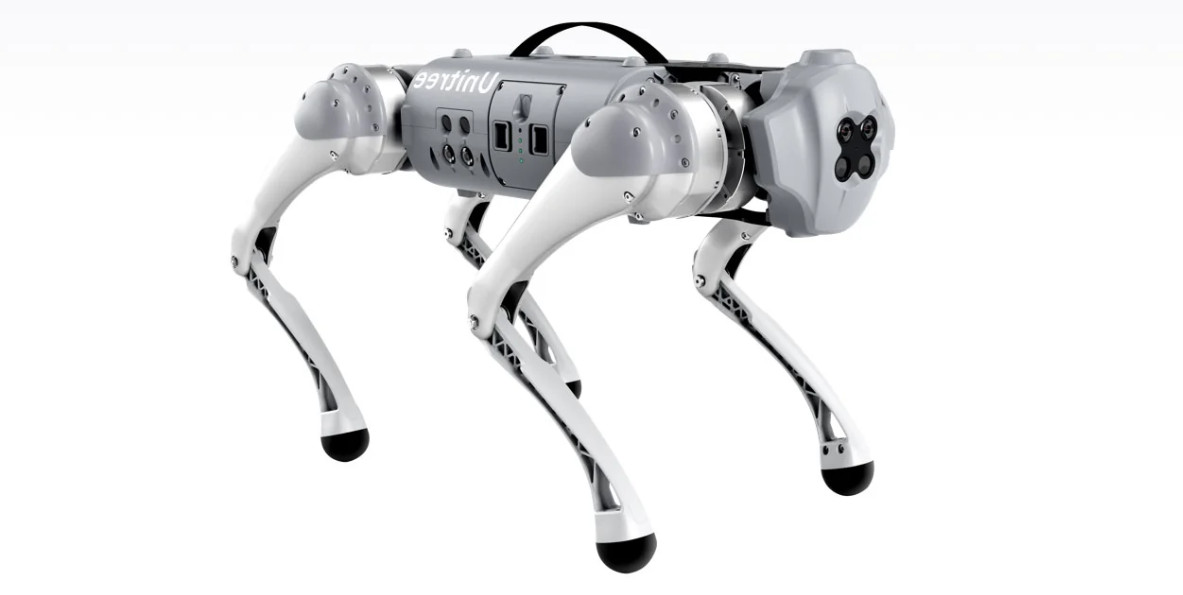
\includegraphics[width=\linewidth]{img/einleitung/go1-ad-foto}}
    \caption[Verkaufsbild des Unitree Go1]{Verkaufsbild des Unitree Go1\footnotemark}\label{fig:go1-ad-foto}
\end{figure}
\footnotetext{\cite{go1-ad-foto}}


Im Bearbeitungszeitraum dieser Arbeit ist bereits der Nachfolger in der Baureihe \emph{GO} erschienen -- der Unitree GO2,
welcher durch einen noch günstigeren Einstiegspreis von beworbenen \num{1600} \gls{usd} und den Spezifikationen nach zu urteilen
deutlich verbesserten und erweiterten Funktionalitäten als verbraucherfreundliche Alternative zum \gls{go1} angesehen
werden kann.

\subsection{Vorgehensweise}
\label{subsec:intro-vorgehensweise}

Die folgende Arbeit besteht im Grunde aus vier Teilen, den Grundlagen, der Roboterarchitektur, der Analyse des Roboters
und der Funktionserweiterung des Roboters.
Im ersten Teil, den Grundlagen, soll ein allgemeiner Überblick über das Thema Robotik geschaffen werden, der besonders zur
Einordnung des bearbeiteten \gls{go1} in das Feld allgemein dienen soll.
Darauf folgend wird der aktuelle Stand der Forschung und Industrie im Bereich der abgegrenzten Einordnung des Roboters
in die Robotik gezeigt werden.
Hierfür werden zuerst Arbeiten und Veröffentlichungen sowie Produkte im Bereich der Quadruped Robotik und deren Nutzung
gezeigt.
Danach sollen Ressourcen zum \gls{go1} gezeigt werden, die besonders in der Arbeit mit dem Roboter nützlich sind.
Hierunter fallen nicht nur offizielle Ressourcen, sondern auch verwandte Veröffentlichungen und ungeprüfte Ressourcen
aus nicht-akademischem Umfeld, die aufgrund ihres Umfangs dennoch beachtet werden sollten.
Als Abschluss der Grundlagen werden einige Herausforderungen bei der Arbeit mit dem \gls{go1} aufgelistet, die zu Teilen
im Laufe der Arbeit wieder aufgegriffen werden sollen.

Nach Schaffung der Grundlagen zum Thema Robotik allgemein und den spezielleren Informationen zum \gls{go1} wird dieser
genauer betrachtet.
Hierfür wird der Aufbau des Roboters detailliert beschrieben und anhand von Grafiken und Fotografien veranschaulicht.
Nach einem Überblick zum Aufbau des Roboters werden die verbauten mechanischen Komponenten, die Sensorik und die Recheneinheiten
dokumentiert.
Darauf folgt eine genaue Analyse der verbauten Recheneinheiten, deren einzelner Funktionen und der Kommunikation dieser
untereinander und mit dem Nutzer.
Zuletzt sollen die technischen Limitierungen des \gls{go1} gezeigt werden.

Aufbauend auf dem geschaffenen Wissen zum Aufbau des Roboters wird in der Analyse des Roboters die Funktion dessen
dokumentiert.
Nach der Beschreibung der Inbetriebnahme des \gls{go1} wird der Großteil der Funktionen, die ab Werk möglich sind,
dokumentiert und bewertet.
Als Ergänzungen werden Funktionen, die im Rahmen der Arbeit nicht getestet werden konnten, noch aufgelistet.

Zum Abschluss werden einige Funktionen aus den vorigen Kapiteln aufgegriffen und erweitert.
Es werden nützliche Funktionen zum realen Einsatz des Roboters entwickelt, als auch Möglichkeiten zur Eliminierung oder
Relativierung einiger Limitierungen gezeigt.
Diese sollen dann noch in die Zielsetzung der Arbeit eingeordnet werden, worauf die Arbeit mit dem \gls{go1} noch einmal
final bewertet werden soll.

\subsection{Zielsetzung}
\label{subsec:zielsetzung}

Folgendes Kapitel soll die Erarbeitungen im Rahmen dieser Arbeit eingrenzen und die Ziele klar definieren.
Eine Evaluation des Erreichten findet am Ende dieser Arbeit statt.

\myparagraph{Ziele}

Die Ziele dieser Arbeit leiten sich vom Titel dieser ab -- \emph{\mytitle}.
Die genannte \emph{Integration} des Roboters kann in verschiedenen Aspekte des Hochschul-Ökosystems erreicht werden.
Hierunter gehören die für diese Arbeit relevanten Aspekte \emph{Forschung}, \emph{Lehre} und \emph{Nutzen}.
Die Nutzung des Roboters im Hochschul-Ökosystem soll in dieser Arbeit nur exemplarisch dargestellt werden.
Erarbeitungen, die eine gewisse Einordnung der Erkenntnisse bedürfen, können mögliche Nutzungen exemplarisch darstellen.
Eine tatsächliche Umsetzung eines Projektes anhand des Roboters zur Nutzung auf dem Hochschulgelände ist jedoch nicht
im Rahmen dieser Arbeit umgesetzt.

Der zweite relevante Aspekt des Ökosystems ist die Forschung, welche in Kombination mit der Lehre besonders von der
Anschaffung eines \gls{go1} durch die Hochschule profitieren kann.
Als Grundlage für weitere Arbeiten am Roboter, besonders des Testens der Grenzen, des Erforschens neuer Einsatzmöglichkeiten
oder der Interaktion des Roboters mit dem Menschen, sollen ein Großteil der Funktionen genau getestet und ihre Limitierungen,
wenn vorhanden, dargestellt werden.

Im Bereich der Lehre gilt ein ähnliches Prinzip, die Darstellung der Funktionen und die Dokumentation der Einzelheiten
des Roboters soll es den Lehrenden und Studierenden vereinfachen, Arbeiten und Versuche am Roboter durchzuführen.
Auch die Dokumentation des Aufbaus soll es Neulingen im Bereich der Quadruped Robotik erleichtern, sich einen Überblick über
die Funktion eines solchen Roboters zu verschaffen.

Zusammengefasst gilt diese Arbeit als eine Art \emph{Survey} zum \gls{go1} und dessen Funktionen.
Hierbei wird dieser genau inspiziert, all dessen Komponenten dokumentiert, die wichtigsten Funktionalitäten getestet und
dokumentiert und durch Erweiterungen die gravierendsten Limitierungen des Roboters behoben sowie die einfachsten Anwendungen
dessen erleichtert.

\myparagraph{Abgrenzung}

Der Roboter enthält diverse Vorbereitungen zum Thema \gls{ki}, welche in dieser Arbeit maximal erwähnt werden sollen.
Auch die Umsetzung dieser Funktionen wird nicht dokumentiert.
Unter diese Funktionen fallen Themen wie Kamerabildoptimierung, Umgebungserkennung durch Ultraschall und \gls{lidar},
Objekterkennung durch die diversen Sensoren und Optimierung der Bewegungsabläufe.
Auch die mechanischen und elektrotechnischen Grundlagen der Motorik und des Bewegungsapparats werden nicht weiter
geschildert.
